\documentclass[../main.tex]{subfiles}
\begin{document}
本章主要参考\cite{euclid,geometry,matrix}。

% Reference: https://openstax.org/books/calculus-volume-2/pages/2-2-determining-volumes-by-slicing
% References: https://mathworld.wolfram.com/Prismatoid.html
% https://mathworld.wolfram.com/PlatonicSolid.html
本章讨论 Euclid 三维空间中的位置关系、度量及常见立体。$S_{\text{侧}}$ 表示侧面积，$S_{\text{全}}$ 表示包括底面的总表面积；高一律指垂直距离。
\section{空间位置与度量}
\subsection{点、直线、平面的平行与垂直}\index{点、直线、平面的平行与垂直|hyperpage}
空间两条不同直线可能相交、平行或异面；不相交并不足以推出平行。直线与平面可能包含、平行或相交。
若一条直线不在平面内，且平行于平面内某直线，则它平行于该平面。直线垂直于平面内两条相交直线的方向，当且仅当它垂直于该平面。
两个不同平面平行可用其中两组相交直线分别平行判定；若一个平面包含垂直于另一个平面的直线，则两平面垂直。
\subsection{空间坐标、点积、叉积与混合积}\index{空间坐标、点积、叉积与混合积|hyperpage}
设 $u=(u_1,u_2,u_3)$、$v=(v_1,v_2,v_3)$，则
\begin{gather*}
|u|=\sqrt{u_1^2+u_2^2+u_3^2},\qquad u\cdot v=u_1v_1+u_2v_2+u_3v_3,\\
u\times v=(u_2v_3-u_3v_2,\ u_3v_1-u_1v_3,\ u_1v_2-u_2v_1),\\
u\cdot(v\times w)=\det(u,v,w).
\end{gather*}
非零向量平行当且仅当叉积为零，垂直当且仅当点积为零；三个向量共面当且仅当混合积为零。
\subsection{向量恒等式与空间图形面积}\index{向量恒等式与空间图形面积|hyperpage}
对空间向量 $u,v,w$，Lagrange 恒等式与向量三重积公式为
\begin{align*}
|u\times v|^2&=|u|^2|v|^2-(u\cdot v)^2,\\
u\times(v\times w)&=v(u\cdot w)-w(u\cdot v),\\
(u\times v)\times w&=v(u\cdot w)-u(v\cdot w).
\end{align*}
叉积满足反交换律，且一般不满足结合律，不能省略三重积中的括号。混合积满足
\[
u\cdot(v\times w)=v\cdot(w\times u)=w\cdot(u\times v).
\]
交换任意两个向量会使混合积变号。由 $u,v$ 张成的平行四边形与三角形面积分别为
\[
S_{\text{平行四边形}}=|u\times v|,\qquad
S_{\text{三角形}}=\frac12|u\times v|.
\]
对于三角形 $ABC$，取 $u=B-A,v=C-A$；两个向量共线时，面积为零。
\subsection{空间角与二面角}\index{空间角与二面角|hyperpage}
对方向向量 $u,v\ne0$ 的两直线，其较小夹角 $\theta\in[0,\pi/2]$ 为
\[
\cos\theta=\frac{|u\cdot v|}{|u||v|}.
\]
直线方向为 $v$、平面法向为 $n$ 时，线面角 $\alpha\in[0,\pi/2]$ 满足
\[
\sin\alpha=\frac{|v\cdot n|}{|v||n|}.
\]
两平面的较小夹角 $\beta\in[0,\pi/2]$ 满足 $\cos\beta=|n_1\cdot n_2|/(|n_1||n_2|)$。具体二面角可为钝角：在两指定半平面内，分别取垂直于交线、指向半平面内部的向量 $a,b$，则
\[
\cos\varphi=\frac{a\cdot b}{|a||b|},\qquad0\le\varphi\le\pi.
\]
此处不能随意加绝对值，否则会丢失钝二面角信息。
\subsection{点线面距离与异面直线距离}\index{点线面距离与异面直线距离|hyperpage}
点 $P$ 到过 $P_0$、方向 $v\ne0$ 的直线，以及到平面 $Ax+By+Cz+D=0$ 的距离为
\[
d_{\text{点线}}=\frac{|(P-P_0)\times v|}{|v|},\qquad
d_{\text{点面}}=\frac{|Ax_P+By_P+Cz_P+D|}{\sqrt{A^2+B^2+C^2}}.
\]
平面要求 $(A,B,C)\ne0$。两不平行直线分别过 $P_1,P_2$、方向为 $u,v$ 时，
\[
d=\frac{|(P_2-P_1)\cdot(u\times v)|}{|u\times v|}.
\]
它同时涵盖异面直线与相交直线；平行时分母为零，应改用点到直线距离。平行平面若以相同法向系数写为 $Ax+By+Cz+D_i=0$，则距离为 $|D_1-D_2|/\sqrt{A^2+B^2+C^2}$。
\subsection{垂足、正交分解与平面对称点}\index{垂足、正交分解与平面对称点|hyperpage}
直线 $\ell:P=P_0+tv$（$v\ne0$）上距离点 $Q$ 最近的点为垂足
\[
H=P_0+\frac{(Q-P_0)\cdot v}{|v|^2}v.
\]
相应的正交分解为
\[
Q-P_0=\frac{(Q-P_0)\cdot v}{|v|^2}v+(Q-H),\qquad
(Q-H)\cdot v=0.
\]
平面 $\Pi:n\cdot P+d=0$（$n\ne0$）上的垂足与关于该平面的对称点分别为
\begin{align*}
H&=Q-\frac{n\cdot Q+d}{|n|^2}n,\\
Q'&=2H-Q=Q-2\frac{n\cdot Q+d}{|n|^2}n.
\end{align*}
这里点的加减按位置向量计算；$Q$ 在平面上时有 $H=Q'=Q$。
\subsection{正交投影、平行截面与相似立体}\index{正交投影、平行截面与相似立体|hyperpage}
线段与投影平面的夹角为 $\alpha$，平面图形与投影平面的较小夹角为 $\beta$ 时，
\[
\ell_{\text{投影}}=\ell\cos\alpha,\qquad
S_{\text{投影}}=S\cos\beta.
\]
相似立体的长度比为 $k>0$ 时，表面积比为 $k^2$、体积比为 $k^3$。棱锥或圆锥用平行底面的平面截取，若顶点到截面距离与总高之比为 $t$，则截面面积为底面积的 $t^2$，小锥体积为整体的 $t^3$。
同高立体在每一相应高度的平行截面积均相等，则体积相等（Cavalieri 原理）。
\section{柱、锥、台与球}
\subsection{棱柱与长方体}\index{棱柱与长方体|hyperpage}
底面积为 $B$、高为 $h$ 的棱柱体积为 $V=Bh$。直棱柱底面周长为 $p$ 时，$S_{\text{侧}}=ph$；斜棱柱不能直接以同一式代替侧面积。
长方体三条相邻棱长为 $a,b,c>0$ 时，
\[
V=abc,\qquad S_{\text{全}}=2(ab+bc+ca),\qquad d=\sqrt{a^2+b^2+c^2}.
\]
\begin{center}
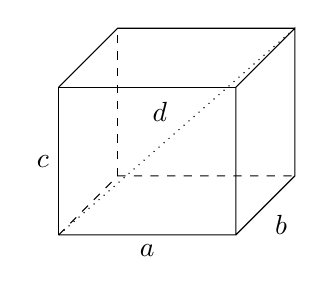
\begin{tikzpicture}[scale=0.75]
\coordinate (A) at (0,0);\coordinate (B) at (3,0);\coordinate (C) at (4,1);\coordinate (D) at (1,1);
\coordinate (E) at (0,2.5);\coordinate (F) at (3,2.5);\coordinate (G) at (4,3.5);\coordinate (H) at (1,3.5);
\draw (A)--node[below]{$a$}(B)--node[below right]{$b$}(C)--(G)--(F)--(B);
\draw (A)--node[left]{$c$}(E)--(F);\draw (E)--(H)--(G);
\draw[dashed] (A)--(D)--(C);\draw[dashed] (D)--(H);
\draw[dotted] (A)--node[above left]{$d$}(G);
\end{tikzpicture}
\end{center}
正方体边长 $a$ 时，体对角线为 $\sqrt3a$，面对角线为 $\sqrt2a$。
\subsection{平行六面体与斜棱柱}\index{平行六面体与斜棱柱|hyperpage}
设平行六面体三条相邻棱向量为 $u,v,w$，且混合积非零，则
\begin{align*}
V&=|u\cdot(v\times w)|,\\
S_{\text{全}}&=2\bigl(|u\times v|+|v\times w|+|w\times u|\bigr).
\end{align*}
若棱长分别为 $a=|u|,b=|v|,c=|w|$，且
\[
\alpha=\angle(v,w),\quad\beta=\angle(w,u),\quad\gamma=\angle(u,v),
\]
则
\[
V=abc\sqrt{1+2\cos\alpha\cos\beta\cos\gamma
-\cos^2\alpha-\cos^2\beta-\cos^2\gamma}.
\]
对于实际非退化立体，根号内严格为正；三个夹角须满足向量之间的相容条件，不能任意独立指定。
对棱柱，记底面积为 $B$，底面单位法向为 $\widehat n$，侧棱向量为 $w\ne0$，底面边向量为 $e_i$，则
\[
h=|w\cdot\widehat n|,\qquad V=Bh,\qquad
S_{\text{侧}}=\sum_{i=1}^m|e_i\times w|.
\]
该侧面积公式来自每个侧面平行四边形的面积；侧棱垂直底面时，才化为底面周长乘高。
\subsection{棱锥与棱台}\index{棱锥与棱台|hyperpage}
棱锥体积为 $V=Bh/3$。正棱锥底面周长为 $p$，各侧面三角形的公共斜高为 $\ell$，则
\[
S_{\text{侧}}=\frac12p\ell.
\]
平行底面截得棱台，上下底面积为 $B_1,B_2$、高为 $h$，则
\[
V=\frac h3(B_1+B_2+\sqrt{B_1B_2}).
\]
正棱台上下底周长为 $p_1,p_2$、侧面梯形公共高为 $\ell$ 时，$S_{\text{侧}}=(p_1+p_2)\ell/2$。斜高位于侧面内，不等于立体的垂直高。
\subsection{正棱锥、正棱台的高、斜高与侧棱}\index{正棱锥、正棱台的高、斜高与侧棱|hyperpage}
设正棱锥底面的外接圆、内切圆半径分别为 $R_b,\rho_b$，垂直高为 $h$，侧棱长为 $e$，侧面斜高为 $\ell$，则
\[
e^2=h^2+R_b^2,\qquad \ell^2=h^2+\rho_b^2.
\]
若底面为边长 $a$ 的正 $n$ 边形（$n\ge3$），则
\[
R_b=\frac{a}{2\sin(\pi/n)},\qquad
\rho_b=\frac{a}{2\tan(\pi/n)}.
\]
对由同一正棱锥平行截得的正棱台，设两底的外接圆半径为 $R_1,R_2$、内切圆半径为 $\rho_1,\rho_2$，则
\[
e^2=h^2+(R_1-R_2)^2,\qquad
\ell^2=h^2+(\rho_1-\rho_2)^2.
\]
这里 $e$ 是侧棱长，$\ell$ 是侧面梯形的高；两底须为同一正棱锥的平行截面。
\subsection{拟柱体的体积公式}\index{拟柱体的体积公式|hyperpage}
设凸多面体的全部顶点位于两个平行平面上，两底面积为 $B_1,B_2$，两平面距离为 $h>0$，中间高度处的平行截面积为 $B_m$，则
\[
V=\frac h6(B_1+4B_m+B_2).
\]
这称为拟柱体公式。底面允许退化为点或线；$B_m$ 是实际中截面积，一般不等于 $(B_1+B_2)/2$。
\begin{align*}
\text{棱柱：}\quad B_1=B_2=B_m=B&\ \Longrightarrow\ V=Bh,\\
\text{棱锥：}\quad B_1=B,\ B_2=0,\ B_m=B/4&\ \Longrightarrow\ V=Bh/3.
\end{align*}
棱台的中截面积为 $B_m=(\sqrt{B_1}+\sqrt{B_2})^2/4$，代入后得到前述棱台公式；该中截面积关系不能直接推广到任意拟柱体。
\subsection{直圆柱、直圆锥与圆台}\index{直圆柱、直圆锥与圆台|hyperpage}
直圆柱半径 $r$、高 $h$ 时，
\[
V=\pi r^2h,\quad S_{\text{侧}}=2\pi rh,\quad S_{\text{全}}=2\pi r(h+r).
\]
直圆锥的母线 $\ell=\sqrt{r^2+h^2}$，满足
\[
V=\frac13\pi r^2h,\quad S_{\text{侧}}=\pi r\ell,\quad S_{\text{全}}=\pi r(\ell+r).
\]
直圆台上下底半径 $R\ge r\ge0$、高 $h>0$，母线 $\ell=\sqrt{h^2+(R-r)^2}$，则
\[
V=\frac{\pi h}3(R^2+Rr+r^2),\quad
S_{\text{侧}}=\pi(R+r)\ell,\quad S_{\text{全}}=S_{\text{侧}}+\pi(R^2+r^2).
\]
\subsection{圆柱、圆锥与圆台的侧面展开}\index{圆柱、圆锥与圆台的侧面展开|hyperpage}
直圆柱侧面沿一条母线剪开后为长方形，长为 $2\pi r$、宽为 $h$。
直圆锥底面半径为 $r>0$、高为 $h>0$、母线为 $\ell=\sqrt{r^2+h^2}$，侧面展开为半径 $\ell$、圆心角 $\varphi$ 的扇形：
\[
\varphi=\frac{2\pi r}{\ell},\qquad \ell\varphi=2\pi r,\qquad
\frac12\ell^2\varphi=\pi r\ell.
\]
直圆台两底半径为 $R>r>0$、母线为 $\ell$，侧面展开为同心扇环：
\begin{align*}
L_{\text{外}}&=\frac{R\ell}{R-r}, &
L_{\text{内}}&=\frac{r\ell}{R-r}, &
\varphi&=\frac{2\pi(R-r)}{\ell},\\
L_{\text{外}}-L_{\text{内}}&=\ell, &
L_{\text{外}}\varphi&=2\pi R, &
L_{\text{内}}\varphi&=2\pi r.
\end{align*}
\par\begin{samepage}
\begin{center}
\begin{tikzpicture}[scale=0.85]
\draw (0,0)--(2.7,0) arc[start angle=0,end angle=70,radius=2.7]--cycle;
\draw (0.55,0) arc[start angle=0,end angle=70,radius=0.55];
\node at (0.85,0.35) {$\varphi$};
\node[above] at (1.4,0) {$\ell$};
\node at (1.65,1.5) {$2\pi r$};
\node at (1.3,-0.6) {圆锥：扇形};
\begin{scope}[xshift=5.7cm]
\draw (1.1,0)--(2.7,0) arc[start angle=0,end angle=70,radius=2.7]
--(70:1.1) arc[start angle=70,end angle=0,radius=1.1];
\draw[dashed] (0,0)--(1.1,0) (0,0)--(70:1.1);
\draw (0.5,0) arc[start angle=0,end angle=70,radius=0.5];
\node at (0.72,0.3) {$\varphi$};
\node[above] at (1.9,0) {$\ell$};
\node[rotate=70,above] at (70:1.85) {$L_{\text{外}}-L_{\text{内}}$};
\node at (2,1.8) {$2\pi R$};
\node at (1.1,0.95) {$2\pi r$};
\node at (1.3,-0.6) {圆台：扇环};
\end{scope}
\end{tikzpicture}
\end{center}
图中圆弧标注表示弧长，$\varphi$ 使用弧度。$R=r$ 时应改用圆柱的长方形展开图；$r=0$ 时退化为圆锥扇形。
\par\end{samepage}
\subsection{球、球冠与球带}\index{球、球冠与球带|hyperpage}
半径 $R>0$ 的球体及球面满足
\[
V=\frac43\pi R^3,\qquad S=4\pi R^2.
\]
距球心 $d$ 的截平面与球面的交圆半径为 $\rho=\sqrt{R^2-d^2}$（$0\le d\le R$）。高为 $h$ 的球冠（$0\le h\le2R$）有
\[
S_{\text{曲面}}=2\pi Rh,\qquad
V=\pi h^2\left(R-\frac h3\right),\qquad\rho^2=2Rh-h^2.
\]
球冠曲面面积不含截口圆盘。两平行截面间的球带曲面面积同样为 $2\pi Rh$；若两截口圆半径为 $a,b$，截得球体部分的体积为
\[
V=\frac{\pi h}6(3a^2+3b^2+h^2).
\]
\subsection{球与内接、外切立体}\index{球与内接、外切立体|hyperpage}
正方体棱长为 $a$ 时，外接球半径与内切球半径分别为
\[
R_{\text{外}}=\frac{\sqrt3}{2}a,\qquad
r_{\text{内}}=\frac a2.
\]
直圆柱的两个底面圆周都在半径为 $R$ 的球面上，设底面半径为 $r$、高为 $h$，则
\[
r^2+\frac{h^2}{4}=R^2.
\]
球心位于圆柱轴线的中点；不能将圆柱高误当成轴截面直角三角形的一条直角边，应取 $h/2$。
直圆锥底面半径为 $r>0$、高为 $h>0$、母线为 $\ell=\sqrt{r^2+h^2}$，则
\[
R_{\text{外接球}}=\frac{h^2+r^2}{2h},\qquad
\rho_{\text{内切球}}=\frac{rh}{r+\ell}
=\frac{r(\ell-r)}{h}.
\]
外接球通过锥顶和底面圆周，其球心在轴线上，距底面沿锥顶方向的有向坐标为 $(h^2-r^2)/(2h)$，该值可以为负。
内切球与底面及侧面相切，其轴截面为等腰三角形的内切圆。
\par\begin{samepage}
\begin{center}
\begin{tikzpicture}[scale=0.8]
\draw (0,0) circle[radius=2.1];
\draw (-1.68,-1.26) rectangle (1.68,1.26);
\draw[dashed] (0,-1.26)--(0,1.26);
\draw (0,0)--node[above left]{$R$}(1.68,1.26);
\draw (0,0)--node[below]{$r$}(1.68,0);
\node[right] at (1.68,0.65) {$h/2$};
\fill (0,0) circle(1.5pt) node[below left]{$O$};
\node at (0,-2.65) {球内接圆柱的轴截面};
\begin{scope}[xshift=6.8cm,yshift=-1.4cm]
\draw (-1.8,0)--(0,2.8)--node[right]{$\ell$}(1.8,0)--cycle;
\draw[dashed] (0,0)--node[left,pos=0.8]{$h$}(0,2.8);
\draw (0,0)--node[below]{$r$}(1.8,0);
\draw (0,0.983) circle[radius=0.983];
\fill (0,0.983) circle(1.5pt);
\draw (0,0.983)--node[above]{$\rho$}(0.983,0.983);
\node at (0,-1.25) {圆锥内切球的轴截面};
\end{scope}
\end{tikzpicture}
\end{center}
轴截面中，圆柱对应矩形，圆锥对应等腰三角形；图中的 $\rho$ 为内切球半径。
\par\end{samepage}
\section{多面体与空间解析几何}
\subsection{凸多面体与五种正多面体}\index{凸多面体与五种正多面体|hyperpage}
凸多面体满足 Euler 公式 $V-E+F=2$，此处 $V$ 表示顶点数而非体积。若每个面为正 $p$ 边形、每个顶点汇聚 $q$ 个面，则
\[
pF=2E=qV,\qquad\frac1p+\frac1q>\frac12.
\]
\par\begin{samepage}
凸正多面体只有以下五种：
\begin{center}
\begin{tabular}{c|c|c|c|c}
名称 & $(p,q)$ & 顶点 $V$ & 边 $E$ & 面 $F$\\\hline
正四面体 & $(3,3)$ & $4$ & $6$ & $4$\\
正六面体 & $(4,3)$ & $8$ & $12$ & $6$\\
正八面体 & $(3,4)$ & $6$ & $12$ & $8$\\
正十二面体 & $(5,3)$ & $20$ & $30$ & $12$\\
正二十面体 & $(3,5)$ & $12$ & $30$ & $20$
\end{tabular}
\end{center}
有孔或其他拓扑类型的多面体表面不能直接套用右端为 $2$ 的公式。
\par\end{samepage}
\subsection{五种正多面体的表面积与体积}\index{五种正多面体的表面积与体积|hyperpage}
设所有棱长均为 $a>0$，总表面积为 $S$、体积为 $V$，则
\begin{center}
\renewcommand{\arraystretch}{1.6}
\begin{tabular}{c|c|c}
名称 & 总表面积 $S$ & 体积 $V$\\\hline
正四面体 & $\sqrt3a^2$ & $\dfrac{\sqrt2}{12}a^3$\\
正六面体 & $6a^2$ & $a^3$\\
正八面体 & $2\sqrt3a^2$ & $\dfrac{\sqrt2}{3}a^3$\\
正十二面体 & $3\sqrt{25+10\sqrt5}\,a^2$ & $\dfrac{15+7\sqrt5}{4}a^3$\\
正二十面体 & $5\sqrt3a^2$ & $\dfrac{5(3+\sqrt5)}{12}a^3$
\end{tabular}
\end{center}
对任一正多面体，若内切球半径为 $r$，以球心和各面组成棱锥可得 $V=rS/3$。
\subsection{四面体体积与正四面体}\index{四面体体积与正四面体|hyperpage}
对不共面的 $A,B,C,D$，四面体体积为
\[
V_{ABCD}=\frac16|\overrightarrow{AB}\cdot(\overrightarrow{AC}\times\overrightarrow{AD})|
=\frac13S_{ABC}h_D.
\]
若总表面积为 $S$、内切球半径为 $r$，则 $r=3V/S$。正四面体棱长 $a$ 时，
\[
S=\sqrt3a^2,\qquad V=\frac{\sqrt2}{12}a^3,\qquad
R=\frac{\sqrt6}4a,\qquad r=\frac{\sqrt6}{12}a.
\]
$R$ 为外接球半径，$r$ 为内切球半径，两者不能与球冠中的截口半径混淆。
\subsection{四面体的重心、分体积与对棱公式}\index{四面体的重心、分体积与对棱公式|hyperpage}
设 $A,B,C,D$ 不共面，四面体重心为
\[
G=\frac{A+B+C+D}{4}.
\]
若 $M=(B+C+D)/3$ 为对面 $BCD$ 的重心，则 $G$ 在线段 $AM$ 内，且 $AG:GM=3:1$。
重心与四个面组成的小四面体满足
\[
V_{GABC}=V_{GABD}=V_{GACD}=V_{GBCD}=\frac14V_{ABCD}.
\]
设一对对棱 $AB,CD$ 长分别为 $a,b$，所在直线的距离为 $d$，较小夹角为 $\theta\in(0,\pi/2]$，则
\[
V_{ABCD}=\frac16abd\sin\theta.
\]
非退化四面体的对棱所在直线为异面直线；其中 $d$ 是两条直线的公垂线段长，不是任意两个端点之间的距离。
\par\begin{samepage}
\subsection{直线、平面、球面与常见曲面}\index{直线、平面、球面与常见曲面|hyperpage}
过 $P_0$、方向为 $v\ne0$ 的直线为 $P=P_0+tv$（$t\in\mathbb R$）；过 $P_0$、法向为 $n\ne0$ 的平面为 $n\cdot(P-P_0)=0$。
球心 $O=(x_0,y_0,z_0)$、半径 $R$ 的球面为
\[
(x-x_0)^2+(y-y_0)^2+(z-z_0)^2=R^2.
\]
在球上点 $P_1$ 处的切平面为 $(P_1-O)\cdot(P-P_1)=0$。常见空间曲面还有
\begin{align*}
\frac{x^2}{a^2}+\frac{y^2}{b^2}+\frac{z^2}{c^2}&=1 &&\text{（椭球面，}a,b,c>0\text{）},\\
x^2+y^2&=R^2 &&\text{（圆柱面）},\\
x^2+y^2&=k^2z^2 &&\text{（双圆锥面，}k>0\text{）},\\
z&=\frac{x^2}{a^2}+\frac{y^2}{b^2} &&\text{（椭圆抛物面，}a,b>0\text{）}.
\end{align*}
曲面方程描述边界，不一定描述内部实体；有限圆柱或圆锥还须指定轴向范围。
\par\end{samepage}
\subsection{直线与球的交点、切线与弦长}\index{直线与球的交点、切线与弦长|hyperpage}
球心为 $O$、半径为 $R>0$，直线为 $P=P_0+tv$（$v\ne0$）。球心到直线的距离为
\[
d=\frac{|(O-P_0)\times v|}{|v|}.
\]
当 $d<R$ 时直线与球面交于两点，所截弦长为
\[
L=2\sqrt{R^2-d^2}.
\]
当 $d=R$ 时相切，$d>R$ 时不相交。求交点时令 $m=P_0-O$，代入球面方程得
\[
|v|^2t^2+2(m\cdot v)t+|m|^2-R^2=0.
\]
记 $D=(m\cdot v)^2-|v|^2(|m|^2-R^2)$，则 $D\ge0$ 时
\[
t_{1,2}=\frac{-m\cdot v\pm\sqrt D}{|v|^2},\qquad
P_{1,2}=P_0+t_{1,2}v.
\]
这里 $D$ 是通常二次方程判别式的四分之一，且 $D=|v|^2(R^2-d^2)$；$D=0$ 时两交点重合为切点。
\par\pagebreak[0]
\begin{samepage}
\subsection{两球相交与交圆}\index{两球相交与交圆|hyperpage}
设两球球心为 $O_1,O_2$，半径为 $R_1,R_2>0$，球心距 $d=|O_2-O_1|>0$。
\[
\begin{array}{c|c}
\text{条件}&\text{两球面的关系}\\\hline
d>R_1+R_2&\text{外离，无交点}\\
d=R_1+R_2&\text{外切，一个交点}\\
|R_1-R_2|<d<R_1+R_2&\text{相交于一个圆}\\
d=|R_1-R_2|&\text{内切，一个交点}\\
0<d<|R_1-R_2|&\text{内含且无交点}
\end{array}
\]
在相交于圆的情形，令 $e=(O_2-O_1)/d$，则交圆所在平面、圆心 $C$ 与半径 $\rho$ 为
\begin{align*}
e\cdot(P-O_1)&=x, & x&=\frac{R_1^2-R_2^2+d^2}{2d},\\
C&=O_1+xe, & \rho&=\sqrt{R_1^2-x^2}.
\end{align*}
$x$ 是从 $O_1$ 沿 $O_1O_2$ 方向量取的有向坐标，可能为负；交圆圆心不一定在线段 $O_1O_2$ 上。
相切时 $\rho=0$，交圆退化为一点。若 $d=0$，则两球面在 $R_1=R_2$ 时重合，否则不相交，应单独处理。
\par\end{samepage}
\section{距离行列式与球面几何补充}
球面角约定参见\cite{geometry}，距离行列式可由 Gram 行列式推导，线性代数公式参见\cite{matrix}。
\subsection{四面体的Cayley--Menger行列式}\index{四面体的Cayley-Menger行列式|hyperpage}
四顶点 $P_0,\ldots,P_3$，记 $d_{ij}=|P_i-P_j|$，体积为 $V$。则
\[
288V^2=\det\begin{pmatrix}
0&1&1&1&1\\
1&0&d_{01}^2&d_{02}^2&d_{03}^2\\
1&d_{01}^2&0&d_{12}^2&d_{13}^2\\
1&d_{02}^2&d_{12}^2&0&d_{23}^2\\
1&d_{03}^2&d_{13}^2&d_{23}^2&0
\end{pmatrix}.
\]
对已能实现的欧氏距离，行列式为零对应共面退化。任意六个正数是否能实现为四面体边长，还必须检查面三角不等式及正定性。
\subsection{Gram矩阵与单纯形体积}\index{Gram矩阵与单纯形体积|hyperpage}
对 $n$ 维单纯形的边向量 $v_i=P_i-P_0$，令 $G_{ij}=v_i\cdot v_j$，则
\[
V_n=\frac{\sqrt{\det G}}{n!},\qquad
G_{ij}=\frac{d_{0i}^2+d_{0j}^2-d_{ij}^2}{2}.
\]
$G\succeq0$ 是这些距离在欧氏空间中实现的条件，$G\succ0$ 对应非退化 $n$ 维单纯形。边长公式与坐标体积公式由此统一。
\subsection{球面三角的正弦与余弦定理}\index{球面三角的正弦与余弦定理|hyperpage}
半径 $R$ 上取由劣大圆弧围成的非退化球面三角形。记边弧长除以 $R$ 为 $a,b,c\in(0,\pi)$、相对内角为 $A,B,C$，则
\[
\cos c=\cos a\cos b+\sin a\sin b\cos C,\qquad
\frac{\sin a}{\sin A}=\frac{\sin b}{\sin B}=\frac{\sin c}{\sin C}.
\]
面积为 $S=R^2(A+B+C-\pi)$。这里 $a,b,c$ 是中心角，不能直接把有量纲的弧长代入三角函数。
\subsection{两球交叠体积}\index{两球交叠体积|hyperpage}
两实心球半径 $R,r>0$，球心距 $d$ 满足 $|R-r|<d<R+r$。沿连心线相加两个球冠体积，得
\[
V=\frac{\pi(R+r-d)^2}{12d}
\left[d^2+2d(R+r)-3(R-r)^2\right].
\]
当 $d\ge R+r$ 时交体积为零；当 $d\le|R-r|$ 时为 $4\pi\min(R,r)^3/3$，后者包含同心情形。不能在 $d=0$ 直接使用带 $1/d$ 的部分相交公式。
\clearpage
\end{document}
